\documentclass{bmvc2k}

%% Enter your paper number here for the review copy
% \bmvcreviewcopy{??}

% \usepackage[brazilian]{babel}
\usepackage[utf8]{inputenc}
\usepackage{float}

\title{Project 2 - Appendix 1}

% Enter the paper's authors in order
% \addauthor{Name}{email/homepage}{INSTITUTION_CODE}
\addauthor{Amélia O. F. da S.}{190037971@unb.br}{1}

% Enter the institutions
% \addinstitution{Name\\Address}
\addinstitution{
  Departamento de Ci\^encia da Comptuta\c{c}\~ao\\
  Universidade de Bras\'{\i}lia\\
  Campus Darcy Ribeiro, Asa Norte\\
  Bras\'{\i}lia-DF, CEP 70910-900, Brazil  
}

\runninghead{Oliveira F. da S., Amélia}{Computer Vision Assignment -- \today}

% Any macro definitions you would like to include
% These are not defined in the style file, because they don't begin
% with \bmva, so they might conflict with the user's own macros.
% The \bmvaOneDot macro adds a full stop unless there is one in the
% text already.
\def\eg{\emph{e.g}\bmvaOneDot}
\def\Eg{\emph{E.g}\bmvaOneDot}
\def\etal{\emph{et al}\bmvaOneDot}

%-------------------------------------------------------------------------
% Document starts here
\begin{document}

\maketitle

\section{Describing the maximisation problem}
\subsection{Determinants and scatter}
The determinant of a scatter matrix can be interpreted as a measurement of the total dispersion of that set of data\cite{statanalysis}.
\subsection{LDA}
Given the scatter matrix for variation "between" classes $S_b$ and the scatter matrix for variation "within" classes $S_w$ and assuming the derivative represents the scatter, the ratio to be maximised can be derived as follows:
\begin{equation}
   \begin{split}
      r = \frac{|S_b|}{|S_w|}\\
      r = |S_b||S_w|^{-1} = |S_b||S_w^{-1}|\\
      r = |S_b\ S_w^{-1}|
   \end{split}
\end{equation}

The problem of maximising a matrix's determinant using a linear transformation $WAW^T$ is equivalent to finding the roots of its characteristic polynomial (finding its eigenvalues)\cite{detmax}. Therefore, maximising the $\frac{|S_b|}{|S_w|}$ ratio through a linear transformation is equivalent to finding the \textit{Eigenvectors} $W_i$ of $S_b\ S_w^{-1}$.

\subsection{PCA}
Following the same logic, maximising the scatter $|S|$ with a linear transformation is equivalent to finding the \textit{Eigenvectors} $W$ of $S$.

\section{Example situation for nearest-mean classification misclassifications}

Using LDA to improve nearest-mean classifications might seem redundant at first thought, but there are situations where it fails when used in the original data basis vectors. This generally occurs when variation within axes is significantly different for each of one.

\begin{figure}[H]
   \begin{center}
      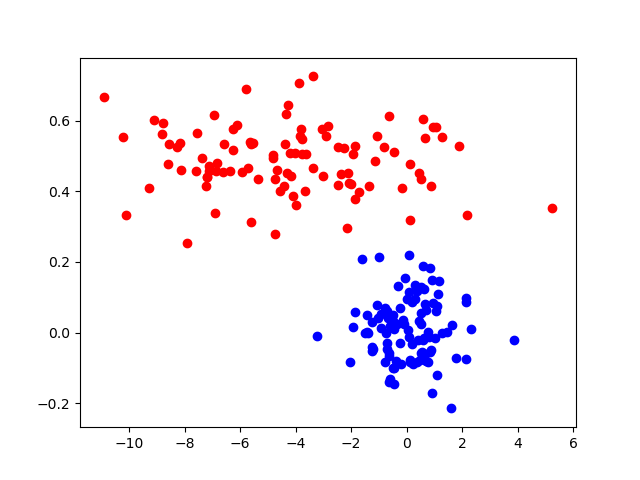
\includegraphics[width=8cm]{figures/Imbalance2D.png}
   \end{center}
   \caption{Heavily asymmetrical variation distribution across axes}
\end{figure}

\begin{figure}[H]
   \begin{center}
      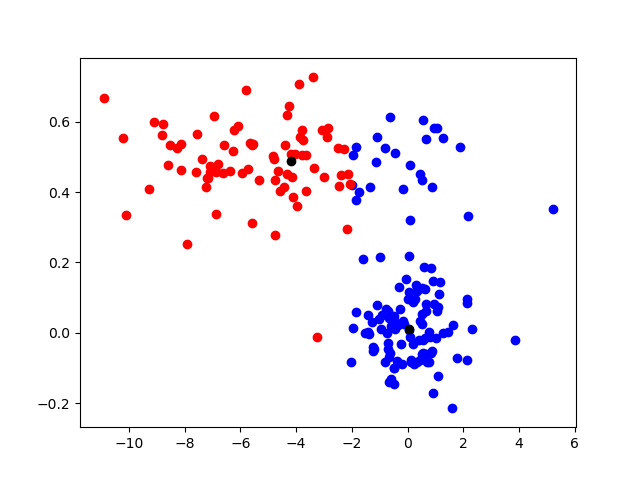
\includegraphics[width=8cm]{figures/MeanMisclassification.png}
   \end{center}
   \caption{Nearest mean misclassifications on the original projection}
\end{figure}

\section{Misclassifications and projections}

Using single-axis projections and thresholding yielded 4 total misclassifications. Analysing the final axis projections allows us to see where the linear classifier failed.

\begin{figure}[H]
   \begin{center}
      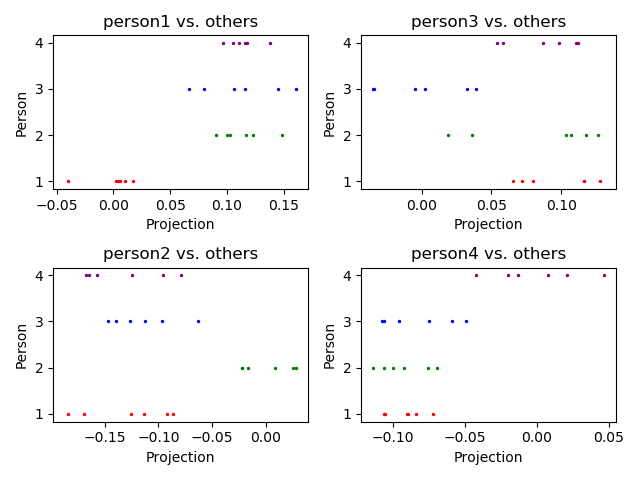
\includegraphics[width=11cm]{figures/ProjectionsNoT.png}
   \end{center}
   \caption{One-against-all axis projections for the four subjects}
\end{figure}
\begin{figure}[H]
   \begin{center}
      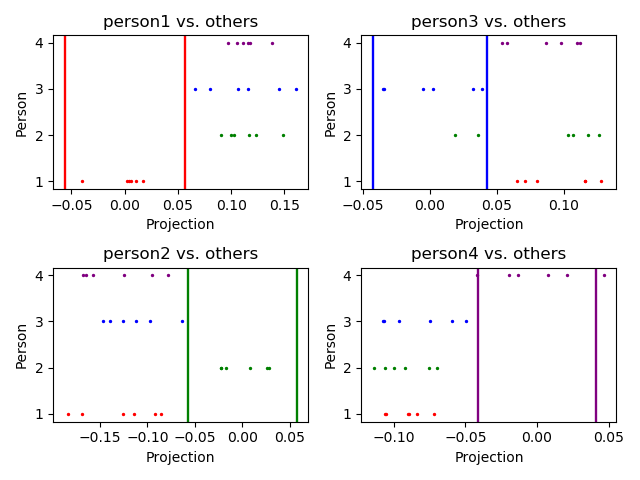
\includegraphics[width=11cm]{figures/ProjectionsT.png}
   \end{center}
   \caption{One-against-all axis projections for the four subjects (including threshold visualisations)}
\end{figure}

Person 3's projection includes two samples from Person 2's set. Person 4's projection excludes 2 of Person 4's own samples.

Improving the threshold calculation and using a more robust classifier would likely solve those problems.

\section{Visual differences evidenced by projection weights}
By comparing each person's most statistically important features with sample projections it is possible to visually understand why those characteristics were chosen for the resulting discrimination.

\begin{figure}[H]
   \begin{center}
      \begin{tabular}{c c}
         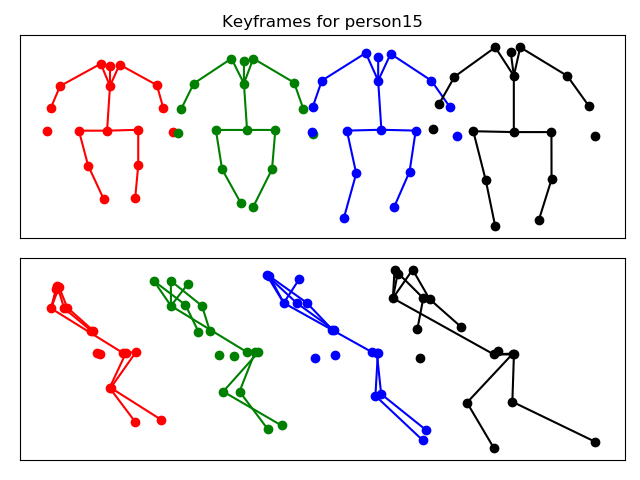
\includegraphics[width=5cm]{figures/walkdata.png}&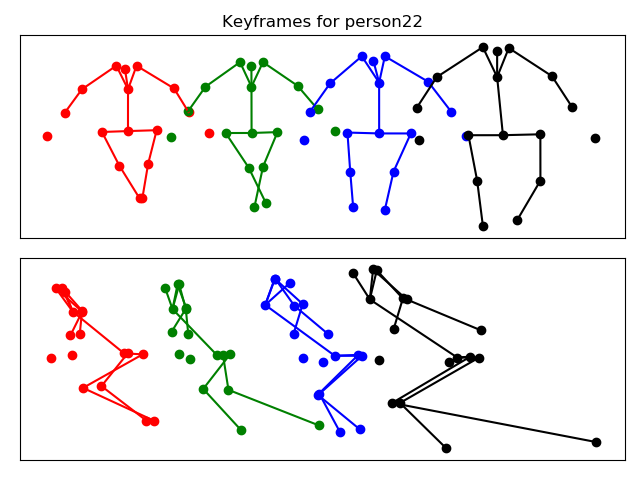
\includegraphics[width=5cm]{figures/walkdatap2.png}\\
         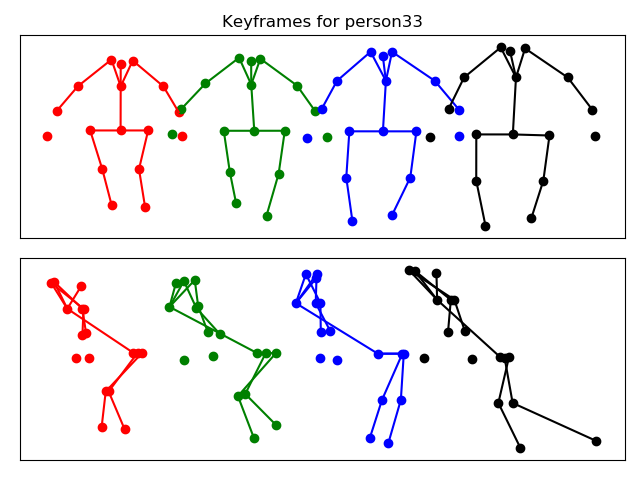
\includegraphics[width=5cm]{figures/walkdatap3.png}&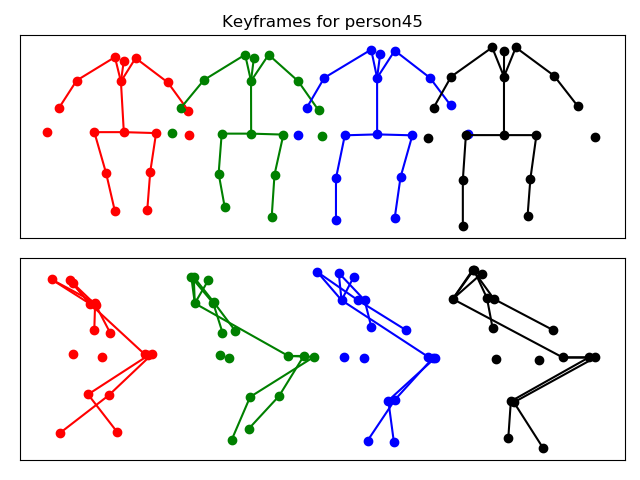
\includegraphics[width=5cm]{figures/walkdatap4.png}
      \end{tabular}
      \caption{Samples from each of the four subjects}
   \end{center}
\end{figure}

\begin{figure}[H]
   \begin{center}
      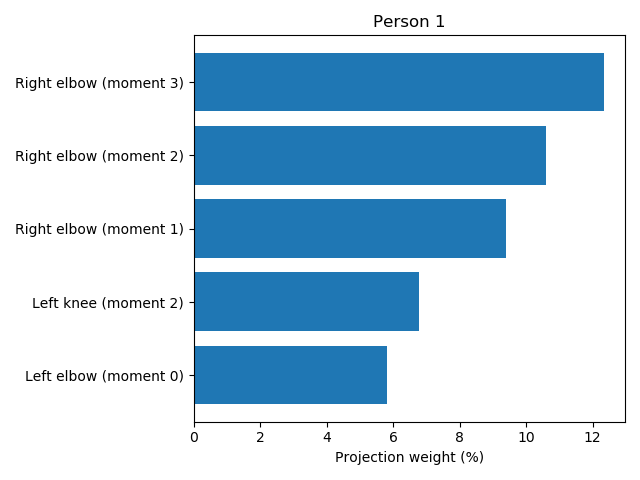
\includegraphics[width=10cm]{figures/person1Imp.png}
      \caption{Person 1's feature importances}
   \end{center}
\end{figure}
Person 1's sample is indeed different from the others on these criteria: their right elbow and left knee stay at a shallower angle than the others.

\begin{figure}[H]
   \begin{center}
      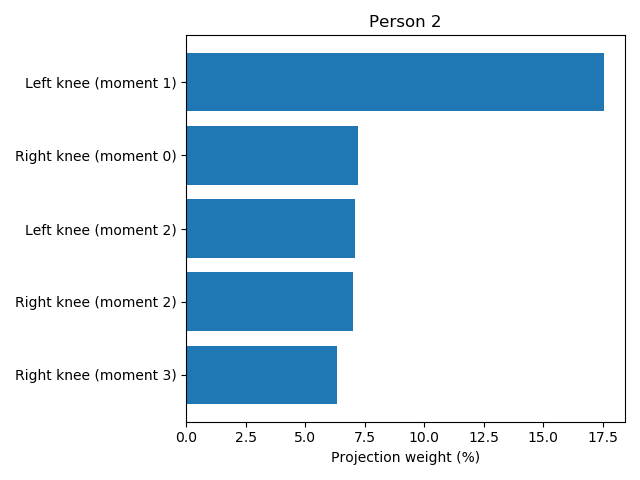
\includegraphics[width=10cm]{figures/person2Imp.png}
      \caption{Person 2's feature importances}
   \end{center}
\end{figure}
Person 2 presents a very idiosyncratic walk pattern, keeping both feet almost in line with each other. This was reflected on their projection axis' feature importances, with knee angles dominating the most important features.

\begin{figure}[H]
   \begin{center}
      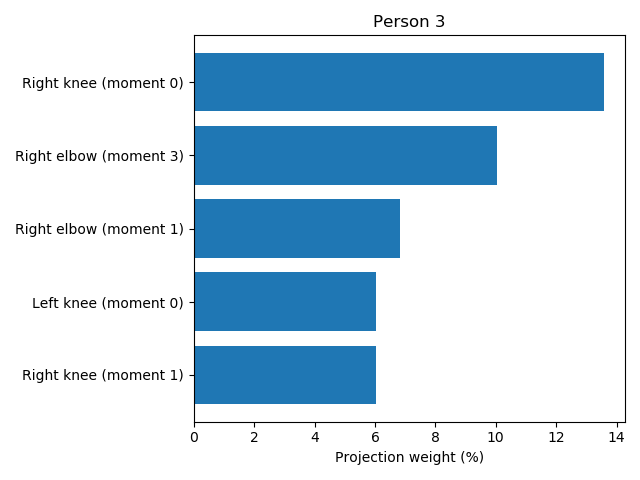
\includegraphics[width=10cm]{figures/person3Imp.png}
      \caption{Person 3's feature importances}
   \end{center}
\end{figure}
Person 3's main feature is their left knee's position at moment 0 (the leftmost/red skeleton on the sample images). It is bent at a shallower angle than all other subjects' samples.

\begin{figure}[H]
   \begin{center}
      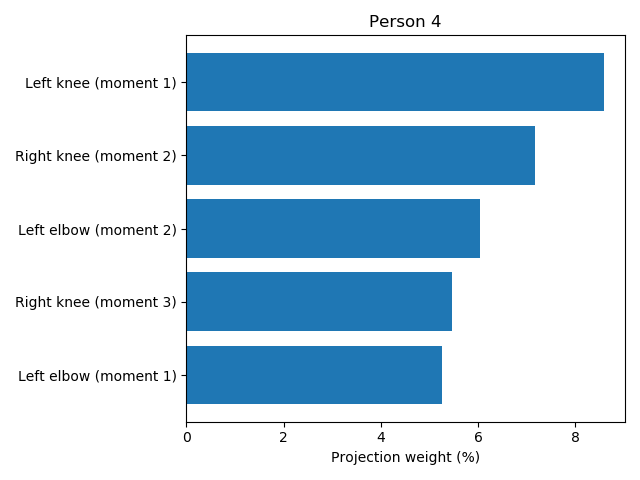
\includegraphics[width=10cm]{figures/person4Imp.png}
      \caption{Person 4's feature importances}
   \end{center}
\end{figure}
Person 4 didn not have many visible peculiar characteristics on their gait, which reflected as a more uniform weight distribution for all features. Their most important feature comprised approximately 8\% of the projection weight, whilst for the other projections, the most important feature was always above 12\% of the projection weight.

\bibliography{refs}

\end{document}
